\documentclass[11pt]{article}
\usepackage{graphicx}
\usepackage{parskip}
\usepackage{multicol}
\usepackage{csquotes}
\usepackage{lipsum}
\usepackage{geometry}
\usepackage[utf8]{inputenc}
\usepackage[english]{babel}

\setlength{\parindent}{2em}
\setlength{\parskip}{1em}
\renewcommand{\baselinestretch}{.90}
\geometry{
 a4paper,
 total={170mm,257mm},
 left=20mm,
 top=20mm,
 }
\graphicspath{ {./} }


\begin{document}
\begin{center}
\section*{American Sign Language with Convolutional Neural Networks}

Addison Boyer \\
Machine Learning (CSCI 547) \\
Fall 2019
\end{center}


\begin{multicols}{2}

\subsection*{1.0 Introduction}
This section provides of an overview of American Sign Language, as well as various computational techniques for Sign Language Recognition.
\\ \\
\textbf{1.1 American Sign Language} 
\par
According to The National Institute on Deafness and Other Communication Disorders (NIDCD) American Sign Language (ASL)
\enquote{is a complete, natural language that has the same linguistic properties as spoken languages, with grammar that differs from English.}  As with most languages, ways of expressing certain ideas in ASL vary from person to person.  For example, within the American Sign Language there exists variations in signing rhythm and pronunciation as well as slang and even the actual signs that are used\textbf{[2]}.  Although ASL, and more generally sign languages certainly vary from region to region, they tend to share two key characteristics.  Namely, sign languages consist of manual and non-manual signing.
\begin{center}
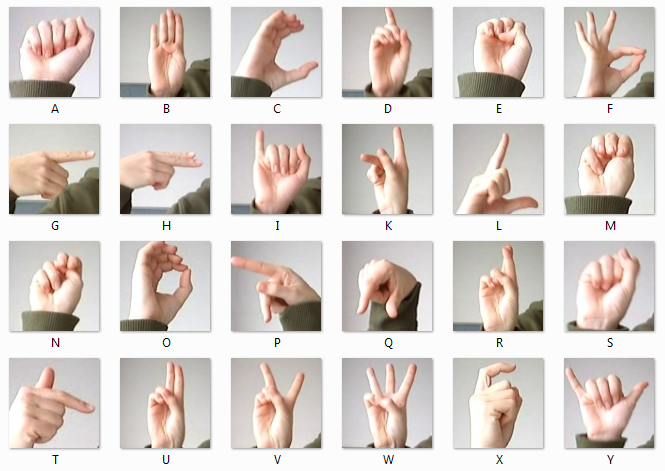
\includegraphics[scale=.45]{amer_sign2}
\textbf{Figure 1.1.1} the ASL alphabet.
\end{center}
\par
Manual signs consist of the positioning of the hands, as well as their orientation, trajectory, and shape.  For example, Figure 1.1.1 shows the manual signs for the alphabet in ASL.  In contrast, non-manual signing consists of the body language, and facial expressions used in conjunction with manual signing.  This component is often helpful to emphasize, or convey the meaning of the manual signs.  However, the manual signs tend to carry the majority of the important lingual information\textbf{[3]}.  With this in mind, researchers generally chose to focus their Sign Language Recognition (SLR) studies on the former. \\ \\
\textbf{1.2 Sign Language Recognition}

\par
Sign Language Recognition is the process of automating the translation of sign language by means of machine learning and/or computer vision techniques.  Without automated forms of SLR, a human interpreter is almost certainly required.  For these very reasons, automated forms of SLR have become extremely important.  Most modern forms of SLR use either vision, or sensor based techniques.  Vision based techniques often cost more computationally, but have the added benefit of not requiring the person signing to wear extra equipment\textbf{[3]}.  Vision based techniques generally only require a camera, a device that anyone with a modern cell phone certainly has.  These types of techniques will be the main focus of the work outlined in this paper.
\par
In this paper I aim to create an ASL sign language recognition system using a Convolutional Neural Network that takes gray-scale images as input, and outputs a classification of those image (0-25 or A-F).  The remainder of this paper is organized into 5 sections consisting of a literature review, methods, results, discussion, and conclusion.

\subsection*{2.0 Literature Review}
This section presents a few examples of works related to sign language recognition using vision-based techniques.  The methods used, as well as the results of the studies are discussed below. \\ \\
\textbf{2.1 SIFT Keypoint Matching}
\par
In \textbf{[4]}, the authors have introduced a sign language classification algorithm that utilizes SIFT keypoints for classification.  Their software pipeline consists of four steps; Image Acquisition, Feature Extraction, Orientation Detection, and Gesture Recognition.  
\par
Images are acquired through a Matlab camera application, and then saved to a directory for later Feature Extraction.  During the feature extraction step, the images are transformed into large collections of local feature vectors.  Then, a series of filtering operations including scale space extrema detection and Keypoint localization are applied to the images.  This filtering reduces the total number of keypoints to process in the remaining steps.  
\par
Next, a consistent orientation is assigned to each Keypoint using local gradient data, and a binning (histogram) approach.  Using this data, Keypoint descriptors are identified in the image.  Lastly, keypoints are calculated for each image in the database, and matched against those of the input image.  The authors of this study concluded that their algorithm did in fact work, and could be used to decode the frames of sign language videos.
\\ \\
\textbf{2.2 Convolutional Neural Networks}
\par
In \textbf{[1]}, the authors have introduced a sign language classification algorithm that utilizes a Convolutional Neural Network for classification.  The network consists of four main parts; The input layer, convolution and pooling layers, and the classification layer.
\par
The input to the CNN is an image of a finger sign in ASL consisting of three 32x32 feature maps, and a single 32x32 feature map for the depth.  Next, these feature maps are transformed by a series of convolutions, and pooling operations.  Finally, these feature maps are flattened and passed into a fully connected feed forward neural network for classification.  This network consists of 2 layers, one hidden layer (128 nodes), and an output layer consisting of 24 nodes (one for each class).

\par
Their network was tested on a data set of 60,000 images (500 for each sign) and excluded J and Z due to their need for motion.  The experiment was run for approximately 250 epochs, or until their network was fully converged.  The ConvNet architecture that they had produced was able to achieve nearly 82\% precision, and 80\% recall.

\subsection*{3.0 Methods}
As previously mentioned, the goal of this work is to create an ASL sign language recognition system that utilizes a Convolutional Neural Network for classification.  The first step in solving this problem was to identify a robust data set to train the network. \\ \\
\textbf{3.1 MNIST Data set for ASL}
\par
The original MNIST data set of handwritten digits is a popular benchmark for image-based machine learning methods.  Researchers have attempted to enhance this dataset and/or provide drop-in replacements which have real world applications.  Among these replacements is the MNIST data set for American Sign Language.
\begin{center}
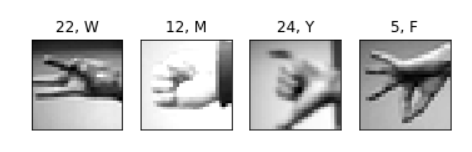
\includegraphics{DataPreview}
\textbf{Figure 3.1.1} A small subset of the MNIST Data set for ASL.
\end{center}
\par
Initially, the data set consisted of 1,704 color images.  The data set has since been augmented to increase the quantity of data.  To accomplish this, a number of transformations were applied to the original images including gray-scaling, cropping around the hand, resizing, filtering, random pixelation, and rotation.  The resulting data set consists of 34,627 gray-scale images, each accompanied by a label identifying it's letter representation.  A small subset of the augmented data set is shown in Figure 3.1.1 above. \\
\\ 
\textbf{3.2 Data Preparation}
\par
The format of the data set closely resembles classic MNIST.  Each training, and test image has a label (0-24) which maps to a letter (A-Z).  There are no labeled images of J=9 or Z=24, as they require gesturing motions beyond the scope of this paper.  The label mappings for the images are shown below in Figure 3.2.1.  
\begin{center}
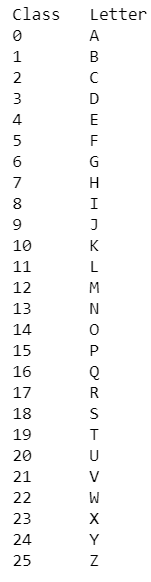
\includegraphics[scale=.50]{Mappings} \\
\textbf{Figure 3.2.1} Letter to Class Mappings.
\end{center}
\par
Each label and image is read in from a .csv file whose rows consist of a single label followed by 784 gray-scale pixel values between 0 and 255.  These pixel values of course make up the 1x28x28 images that will soon become the input to our Convolutional Neural Network.  The data set is separated into training and test cases.  The size of the training data set is 27,455 whereas the size of the test data set used to validate the model is 7,172.  The images comprising the training and test sets were pre-determined, and are not randomly chosen each training session. \\
\\
\textbf{3.3 Network Architecture}
\par
The proposed model is implemented in PyTorch, a machine learning package for Python.  The model takes an array of 1x28x28 images as input.  The input is then passed into a series of 3 convolutional layer blocks.  In each convolutional layer block the feature map(s) are first convolved with a kernel of size 3, and with a padding of 1.  After each convolution a non-linear activation function is applied to each feature map.  This activation function is ReLU or Rectified Linear Unit.  The equation for the rectified linear unit is shown below.
$$
ReLU(x) = \left\{
        \begin{array}{ll}
            0 & \quad x \leq 0 \\
            x & \quad x > 0
        \end{array}
    \right.
$$
\begin{center}
\textbf{Equation 3.3.1} Rectified Linear Unit (ReLU).
\end{center}

\par
Finally, after ReLU activation, each feature map is down sampled via a max pooling operation with a kernel size of 2, and a padding of size 2.  The output is then passed as input to the next convolutional layer block.  After the series of convolutional layer blocks the output is flattened and passed into the fully connected feed forward layer as input.
\par
In the fully connected feed forward layer a series of of linear transformations and ReLU activation's transform the output from the convolutional layer into logits, or probabilities of class membership.  In each hidden layer, the size of the features is nearly halved, and a dropout of approximately 10\% is applied the nodes of that layer.  Adding dropout to the model makes it more robust, and helps the model to not be over fitted.  A summary of the proposed Convolutional Neural Network architecture can be found below in Figure 3.3.1.
\\ \\
\textbf{3.4 Model Training}
\par
Training the model correctly requires the minimization of a cost function with respect to the model's parameters.  The loss function that this model will use is Categorical Cross Entropy loss.  The loss function is used in conjunction with gradient descent in order to adjust the parameters (via back propagation) and train the model.  A batch size of 256 is utilized, and the model is trained for 15 epochs.  Due to the complexity of the network, it is recommended to train the model on a GPU.  Training on a CPU takes approximately 90-120 minutes.
\subsection*{4.0 Results}
\textbf{4.1 Training and Test Set Accuracy}
\par
After training for 15 epochs the model was able to achieve approximately 99.5\% Training set accuracy, and 93\% Test set accuracy.  Training and Test set accuracy by epoch can be found in Figure 4.1.1 below.
\begin{center}
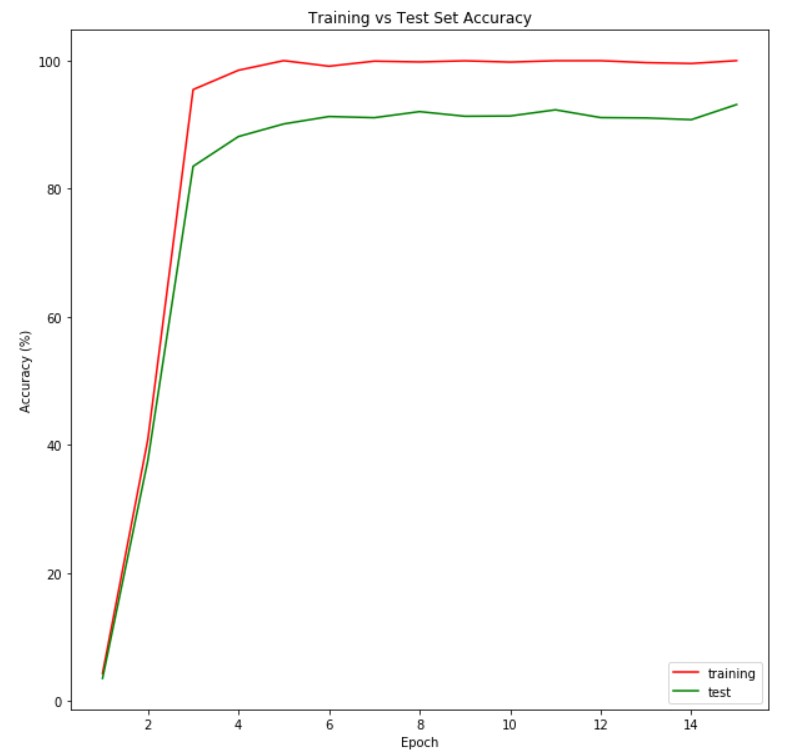
\includegraphics[scale=.5]{TrainingTest}
\textbf{Figure 4.1.1} Training and Test Set Accuracy per Epoch.
\end{center}
\textbf{4.2 Convergence of the Model}
\par
The model has appeared to have converged, as the loss is tending towards 0.  This can be seen in Figure 4.2.1 below
\begin{center}
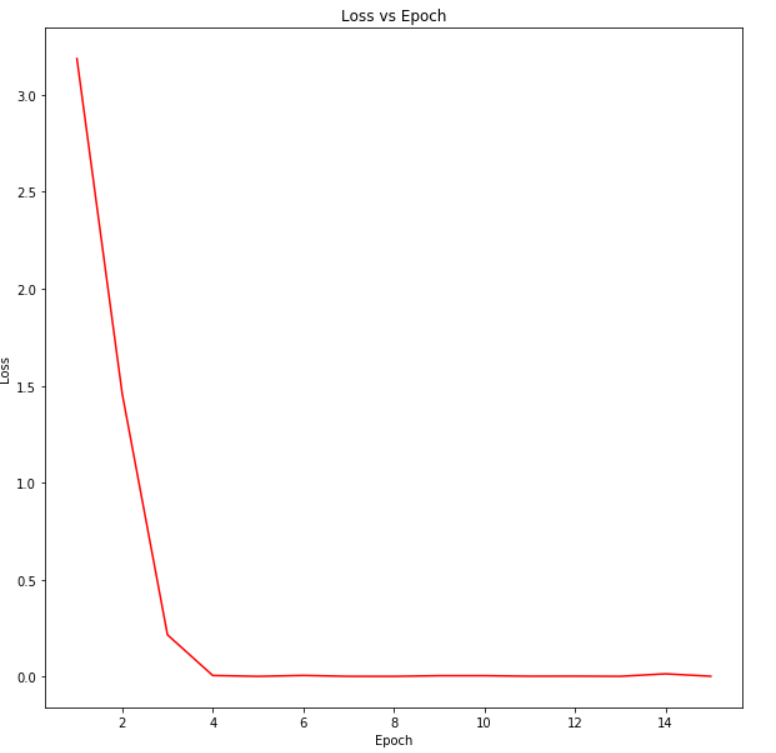
\includegraphics[scale=.5]{LossEpoch}
\textbf{Figure 4.2.1} Categorical Cross Entropy Loss per Epoch.
\end{center}

\textbf{4.3 Precision and Recall}
\par
In order to learn what the model was good at classifying, as well as what it struggled with a confusion matrix was generated.  A graphical representation of the confusion matrix can be found below in Figure 4.3.1.
\begin{center}
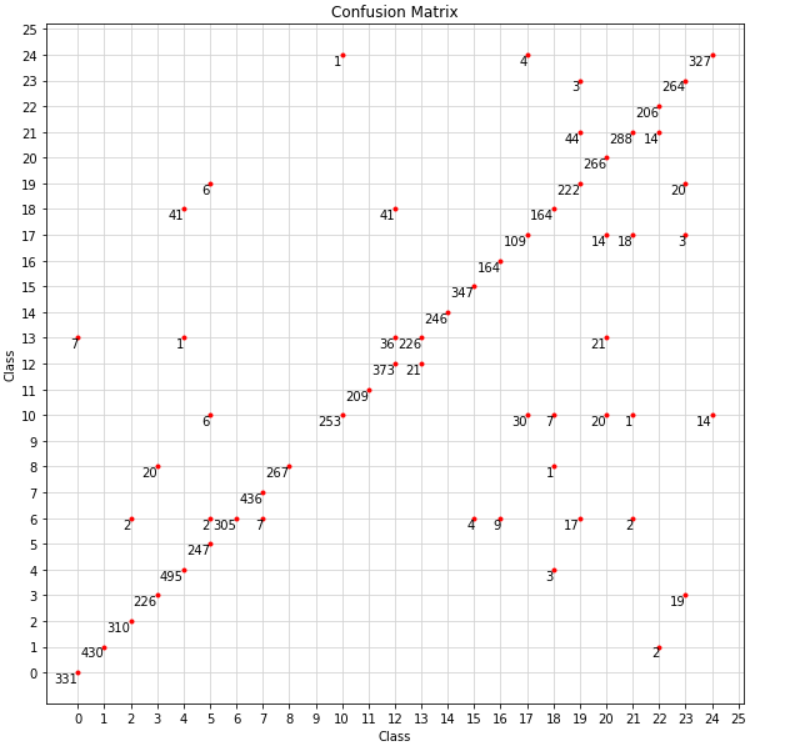
\includegraphics[scale=.50]{ConfusionMatrix}
\textbf{Figure 4.3.1} The Confusion Matrix of the Trained Model.
\end{center}
\begin{center}
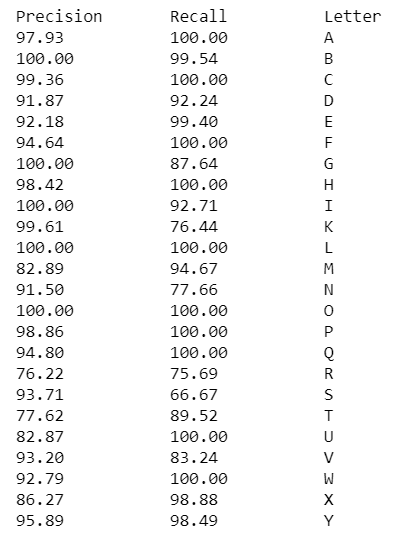
\includegraphics[scale=1.0]{PrecisionRecall} 
\textbf{Figure 4.3.2} Precision and Recall by Letter.
\end{center}
\par
Precision and Recall are good metrics to measure how well the model is performing on certain classifications.  Precision is defined as the total number of correctly classified positive examples, over the total number of positives.  In contrast, Recall is the total number of correctly classified examples, over the total positives.  Precision and Recall calculations are displayed in Figure 4.3.2.


\subsection*{Discussion}

Discussion goes here.

\subsection*{Conclusion}

Conclusion goes here.

\subsection*{References}
\begin{enumerate}
\item[\textbf{[1]}] Ameen, Salem. and Vadera,  Sanil., \enquote{A convolutional neural network to classify American Sign Language fingerspelling from depth and colour images}, \textit{WILEY Expert Systems}, 2016, pp 1-8
\item[\textbf{[2]}] \enquote{American Sign Language.} National Institute of Deafness and Other Communication Disorders, U.S. Department of Health and Human Services, 8 May 2019, www.nidcd.nih.gov/health/american-sign-language.
\item[\textbf{[3]}] Benaddy, Mohamed., El Meslouhi, Othmane., and Hayani, Salma.,\enquote{Arab Sign language Recognition with Convolutional Neural Networks}, \textit{IEEEICCSRE2019}, 2019, pp 1-4
\item[\textbf{[4]}] Goyal, Sakshi., Sharma, Ishita., and Sharma, Shanu., \enquote{Sign Language Recognition System for Deaf and Dumb people}, \textit{International Journal of Engineering Research \& Technology}, 2013, pp 382-387


\end{enumerate}


\end{multicols}


\end{document}